\section{Interfacing with Applications}

\ken{
  Each subsection should be up to 2/3 pages plus have images up to 1/2 page.
  (3.5 pages total.)
  The section should start with a layperson overview of what the domain problem is, what scientists are doing to study the problem.
  The section should then explain how visualization fits in to help.
  Explain the technical solution of how VTK-m was integrated into the system and describe the final result.
  The section may repeat for multiple things that were done.
  For example the fusion reactor could first talk about in situ images and then Poincar\'{e} plots.
  The laser wakefields could talk about deliver of in situ images via Ascent and then about the customized particle advection.
  The final section will be a little different in that it will iterate over multiple science domains.
}

\subsection{Tokamak Fusion Reactor}

\assign{Dave}

(WDMApp/CS Chang/Poincar\'{e})

\subsection{Laser Wakefield Acceleration}\label{sec:warpx}

\assign{Axel, Abhi}

%\defcitealias{FedeliHuebl2022}{Fedeli, Huebl et al. (2022)}
%\citepalias{FedeliHuebl2022}

WarpX is a new particle-in-cell simulation code developed as part of ECP, which was awarded the 2022 ACM Gordon Bell Prize~\cite{FedeliHuebl2022}.
In ECP, WarpX was developed as a fully new code succeeding its predecessor Warp~\cite{Vay2013}, with the goal to study advanced particle acceleration using in laser-driven plasma wakefields, towards future high-energy physics colliders.

Figure~\ref{fig:warpx_lwfa} is an in situ rendering of a \text{staged} laser wakefield accelerator in a boosted reference frame~\cite{Vay2011}.
In the staging approach, a particle beam is accelerated subsequently through multiple plasma elements.
In each stage, an ultra-intense laser pulse is exciting a plasma wakefield.
This depletes the laser pulse's energy to generate very strong electric fields in the plasma wake, which can be used to accelerate an injected electron beam.
The acceleration itself can be three to four orders of magnitude more compact than staging state-of-the-art radio-frequency accelerator elements.
Besides increased beam energy, physicists study how to preserve beam properties essential for transport, focusing (e.g., emittance) and applications (e.g., charge and current).

Shown in figure~\ref{fig:warpx_lwfa} are the strong traversal focusing fields (red-blue) in the plasma stages (gray).
An electron beam (orange-green) is accelerated to the right through multiple stages to high energies.
% Mentioned in Ascent section:
% The scene combines volume rendering (plasma stage), isocontours (focusing fields) and particle glyphs (accelerated beam).

WarpX features advanced techniques such as GPU-acceleration for three vendors, mesh-refinement capabilities, dynamic load balancing, and unique advanced numerical solvers.
WarpX relies on multi-level parallelization: coarse parallelization relies on block-structured domain-decomposition with MPI using the AMReX library~\cite{Zhang2019} and compute acceleration with CUDA/HIP/SYCL or OpenMP, so that simulations are scalable to the world's largest supercomputers.

If WarpX would only rely on traditional post-processing workflows for visualization of the dynamics of Exascale simulations, the resulting multi-PByte scale output per simulation would severely limit the available snapshots and/or level of detail to visualize.
Addressing this need, its situ visualization interfaces to Ascent, for which utility routines were implemented in AMReX, which are specialized in WarpX ``diagnostics'' for application-specific descriptions.
WarpX performs data preparation steps for diagnostics in situ and shares the respective AMReX memory buffers with zero-copy APIs through Conduit with Ascent, rendering with VTK-m in the same domain-decomposition and on the same compute device as the simulation itself.

\begin{figure*}[ht]
  \centering
  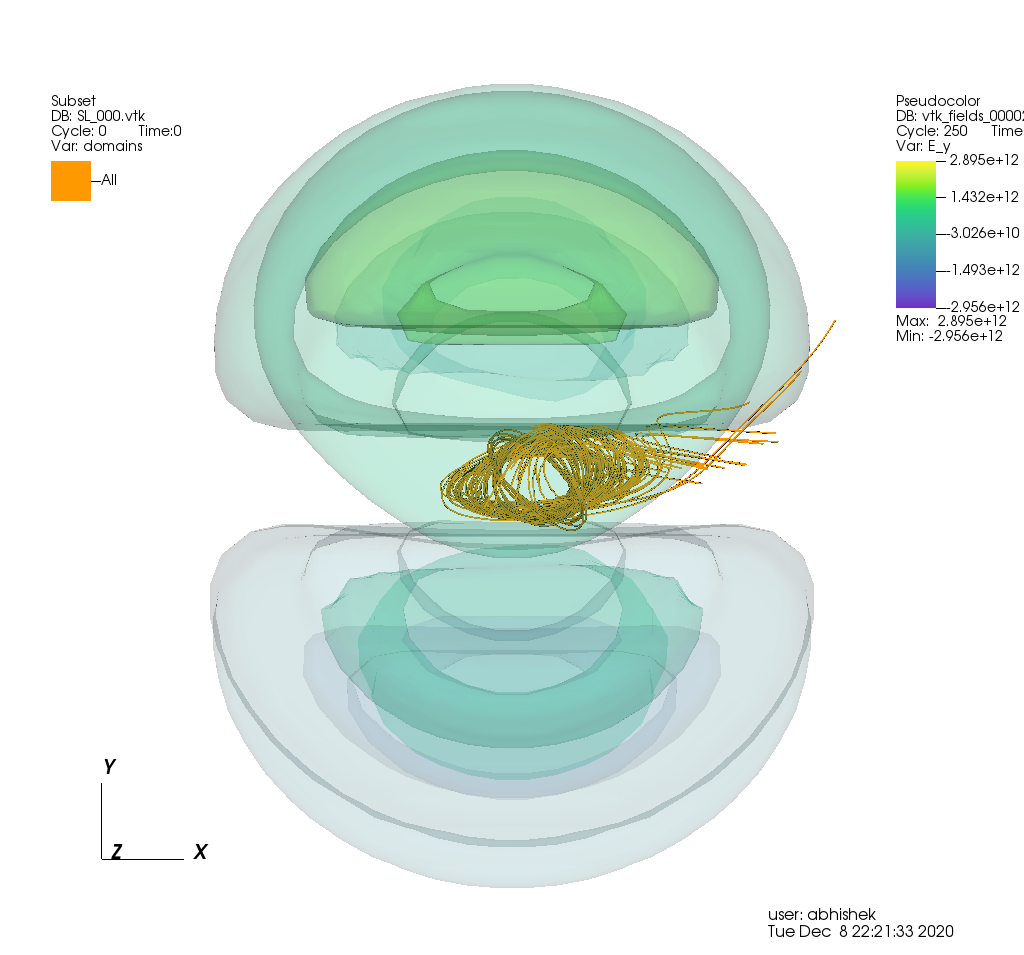
\includegraphics[width=0.49\linewidth]{figures/lwfa_particle_advection_front.png}%
  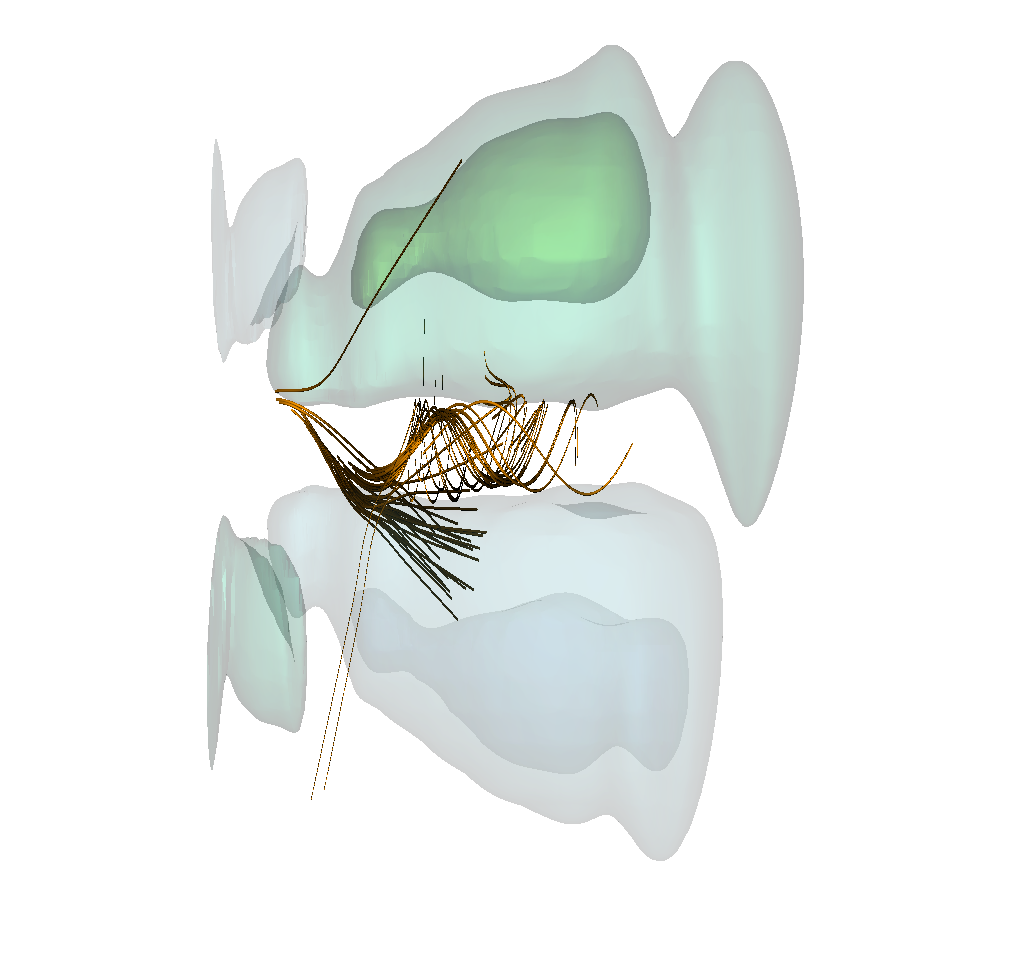
\includegraphics[width=0.49\linewidth]{figures/lwfa_particle_advection_side.png}
  \caption{Side- \& front-view of an laser wakefield with an injected electron bunch.
  Particles are advected from \emph{a single snapshot} of the simulation in VTK-m.}
  \label{fig:lwfa_particle_advection}
\end{figure*}

Realistic visualization of particle trajectories (advection) in a plasma or particle accelerator requires high temporal fidelity in traditional workflows.
With VTK-m, an opportunity to significantly reduce data input for such workflows was identified, making use of a physics-motivated advection algorithm and the slowly changing nature of fields in a wakefield accelerator.

Plasma particles such as electrons and ion are inert and can be relativistic, which effectively changes their mass as they move.
Traditional advection algorithms only made use of local properties of fields, without a history and inert nature of a streamline.
As in a particle-in-cell algorithm, the realistic track of a charged plasma particle can be integrated following the Lorentz-Force, which interpolates six local field components ($E_{x,y,z}, B_{x,y,z}$) and advances the particles momentum (inertia) and position with an explicit forward-iterating scheme.

Using a snapshot of a simulation can then be used to project the particles physical position forward (and backward) for a meaningful time, under the realistic assumption that fields do not change much in time (besides translation along an axis).
Figure~\ref{fig:lwfa_particle_advection} shows such particle trajectories of an off-axis injected electron beam in a wakefield, calculate from a single snapshot, reproducing physical betatron oscillation.

\subsection{Impact Beyond ECP}

\assign{Jay}

%\jay{discuss the applications/use cases outside of ECP}
In addition to the applications mentioned above, VTK-m still serves as the key infrastructure for accelerating data analysis and visualization in various scientific applications through \emph{in situ} approach. This subsection lists several typical examples and illustrates how VTK-m is integrated into \emph{in situ} scientific workflows outside of ECP.


Before being selected as a project in ECP, VTK-m was a core component in Visualization for the Extreme-Scale Scientific Computation Ecosystem (XVis)~\cite{Moreland2019}. 
XVis focused on multiple ways to integrate \emph{in situ} visualization with the simulation, extract key information, and decrease the data size for post-hoc processing.
The ``\emph{in situ} reduction + post hoc'' paradigm is widely adopted in multiple scientific domains, such as probability distribution functions (PDF) extraction of fields in combustion simulation~\cite{7874311}, and binning mechanism to reduce the data size of fusion simulation~\cite{Kress2018}. 


Nyx is a cosmological simulation that aims to solve compressible hydrodynamics with N-body treatment of the dark matter. Each simulation run may contain hundreds of time steps with multiple sets of simulation input parameters. The raw data size is usually hundreds of TBs to several PBs, which causes challenges to process data in post-processing. 
VTK-m is used as \emph{in situ} analysis to extract the statistical properties of the down-sampled data to hugely reduce the size of raw data. The associated statistics model can be used to construct the data based on prior knowledge in post-processing with low data reconstruction error~\cite{Wang2019}.

Eddy detection and tracking plays a key role in the ocean simulation field. Understanding the characteristics of eddies can help scientists to explain the regional air-sea interactions.
VTK-m streamline filter can be used as an \emph{in situ} analysis to generate streamline data used for interactive post-hoc analysis~\cite{Han2022}. With the help of VTK-m, the associated eddy analysis workflow can improve the interaction speed, reduce data storage, and meet the
needs of real-time visual analysis interaction.  
